%%%%%%%%%%%%%%%%%%%%%%%%%%%%%%%%%%%%%%%%%%%%%%%%%%%%%%%%%%%%%%%%%%%%%%%%%%%%%%%%
% ISE Lab -- Topic
% Giovanni Ciatto
% Alma Mater Studiorum - Università di Bologna
% mailto:giovanni.ciatto@unibo.it
%%%%%%%%%%%%%%%%%%%%%%%%%%%%%%%%%%%%%%%%%%%%%%%%%%%%%%%%%%%%%%%%%%%%%%%%%%%%%%%%
%\documentclass[handout]{beamer}\mode<handout>{\usetheme{default}}
%
\documentclass[presentation]{beamer}\mode<presentation>{\usetheme{AMSBolognaFC}}
%\documentclass[handout]{beamer}\mode<handout>{\usetheme{AMSBolognaFC}}
%%%%%%%%%%%%%%%%%%%%%%%%%%%%%%%%%%%%%%%%%%%%%%%%%%%%%%%%%%%%%%%%%%%%%%%%%%%%%%%%
\usepackage{ise-lab-common}
\usepackage{ise-lab-ilp}
% version
\newcommand{\versionmajor}{0}
\newcommand{\versionminor}{1}
\newcommand{\versionpatch}{1}
\newcommand{\version}{\versionmajor.\versionminor.\versionpatch}
%%%%%%%%%%%%%%%%%%%%%%%%%%%%%%%%%%%%%%%%%%%%%%%%%%%%%%%%%%%%%%%%%%%%%%%%%%%%%%%%
\title[\currentLab{} -- Symbolic ML \& ILP]{
    Symbolic Machine Learning and Inductive Logic Programming
}
%
\subtitle{\courseName{} / Module \moduleN{} (\courseAcronym)}
%
\author[\sspeaker{\gcShort}]{\speaker{\gcFull} \\ \gcEmail}
%
\institute[\disiShort, \uniboShort]{\disi{} (\disiShort)\\\unibo}
%
\date[A.Y. \academicYear{} (v.\ \version)]{Academic Year \academicYear{}\\(version \version)}
%
%%%%%%%%%%%%%%%%%%%%%%%%%%%%%%%%%%%%%%%%%%%%%%%%%%%%%%%%%%%%%%%%%%%%%%%%%%%%%%%%
\begin{document}
%%%%%%%%%%%%%%%%%%%%%%%%%%%%%%%%%%%%%%%%%%%%%%%%%%%%%%%%%%%%%%%%%%%%%%%%%%%%%%%%

%/////////
\frame{\titlepage}
%/////////

%%===============================================================================
\section*{Outline}
%%===============================================================================
%
%%/////////
\frame[c]{\tableofcontents[hideallsubsections]}
%%/////////

%===============================================================================
\section{Machine Learning}
%===============================================================================

\begin{frame}[allowframebreaks]
\frametitle{Machine Learning (ML)}
    \begin{block}{A famous definition of ML from \cite{Mitchell1997}:}\itshape
        A computer program is said to learn from \alert{experience $E$} with respect to some class of \alert{tasks $T$} and \alert{performance $P$} if its performance at tasks in $T$, as measured by $P$, improves with experience $E$
    \end{block}

    \begin{alertblock}{Very \textbf{wide} definition, not specifying:}
        %
        \begin{itemize}
            \item what are the possible tasks?
            \item how performance is measured for a given task?
            \item what is experience?
            \item how / when experience should be provided to programs?
            \item what parts of the program are supposed to change via learning?
            \item under which form learnt information is represented?
        \end{itemize}
    \end{alertblock}
\end{frame}

\begin{frame}[allowframebreaks]
\frametitle{Many ways to categorise ML}
    \begin{block}{Supervised, unsupervised, reinforcement learning}
        \begin{itemize}
            \item \textbf{Supervised} learning:
            %
            \begin{itemize}
                \item[$T$] $=$ approximation for unknown \alert{relation}  
                \item[$E$] $=$ a statistically-relevant \alert{sample} of that relation
                \item[$P$] $=$ a \alert{quality measure} for the approximation
            \end{itemize}

            \item \textbf{Unsupervised} learning:
            %
            \begin{itemize}
                \item[$E$] $=$ \alert{set} of \alert{homogeneous} data 
                \item[$T$] $=$ \alert{partitioning} of data into multiple sets
                \item[$P$] $=$ \alert{optimality criterion} intensionally describing the partitioning 
            \end{itemize} 

            \item \textbf{Reinforcement} learning:
            %
            \begin{itemize}
                \item[$T$] $=$ letting agents choose actions in states  
                \item[$E$] $=$ \alert{reward} received for achieving a goal 
                \item[$P$] $=$ \alert{optimality criterion} for the policy
            \end{itemize} 
        \end{itemize}
    \end{block}

    \begin{block}{Symbolic vs. sub-symbolic learning}
        \begin{itemize}
            \item depends on whether the learnt information can be \alert{symbolically} represented or not
        \end{itemize}
    \end{block}

    \begin{block}{On-line vs. off-line learning}
        \begin{description}
            \item[Off-line] $\approx$ learning occurs \alert{before} operation
            \item[On-line] $\approx$ learning occurs \alert{during} operation
        \end{description}
    \end{block}
    
    \begin{center}
        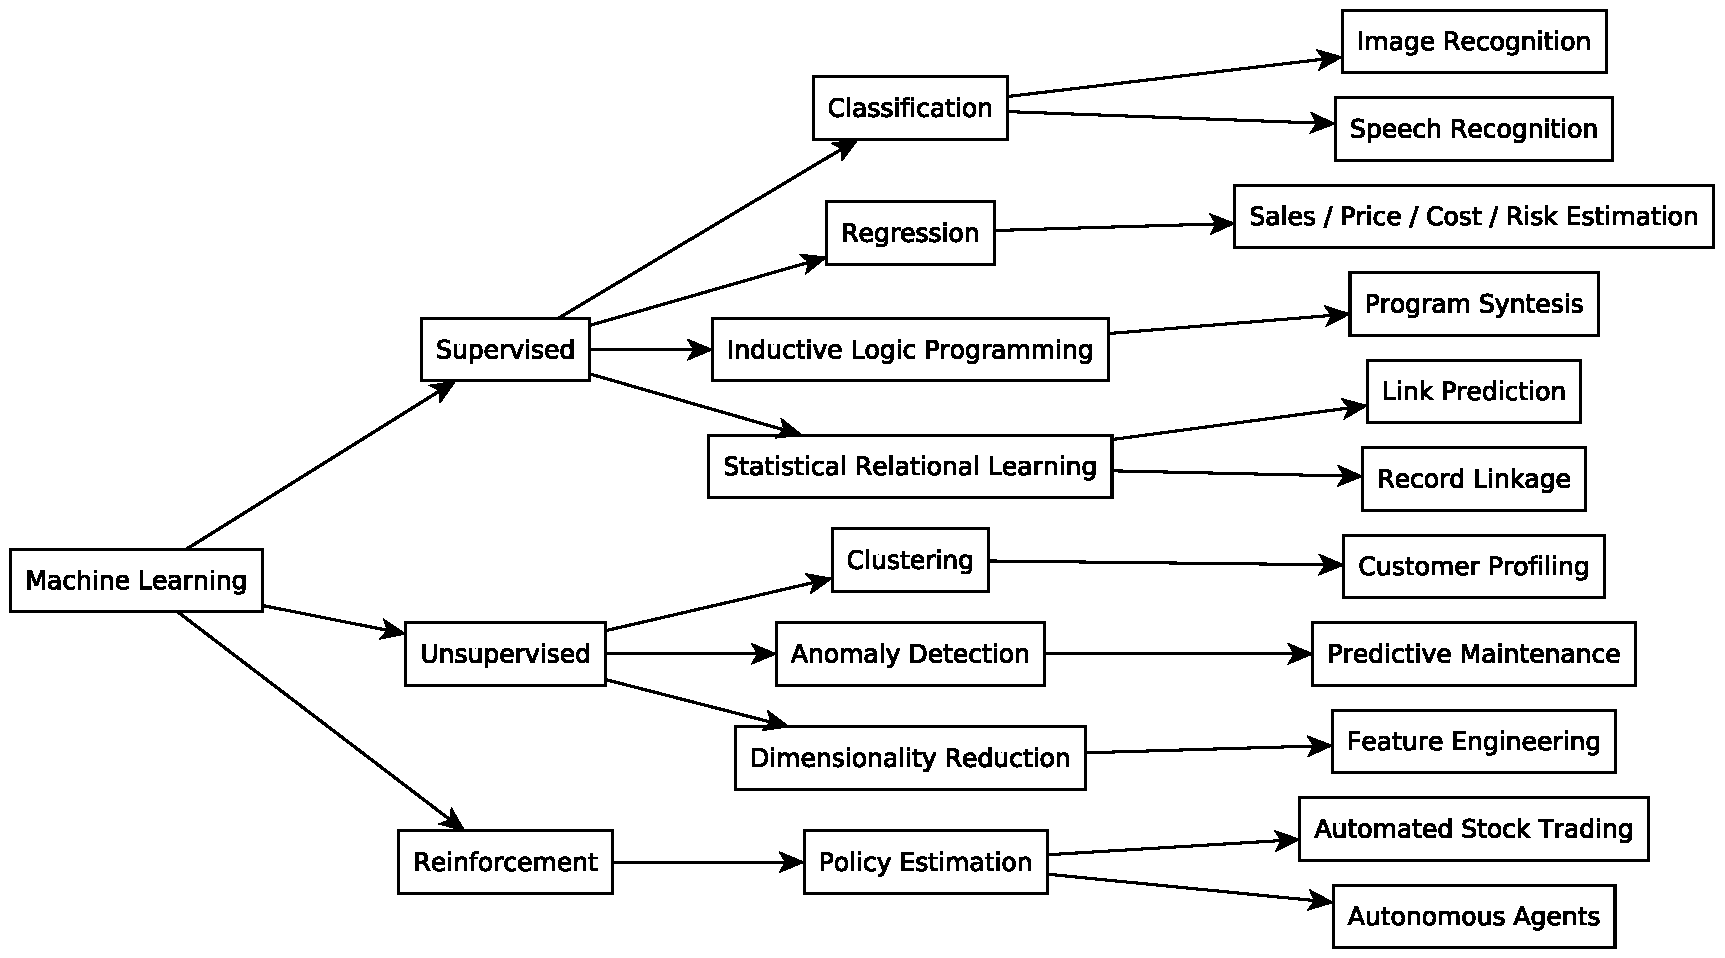
\includegraphics[width=.7\linewidth]{figures/ml-taxonomy.pdf}
    \end{center}
\end{frame}

%===============================================================================
\section{Symbolic Machine Learning}
%===============================================================================

\begin{frame}[allowframebreaks]
\frametitle{Symbolic Supervised Learning}

    \begin{block}{Insights}
        \begin{itemize}
            \item Aims at learning a \alert{relation from examples} (supervised)
            \item The learnt relation is a \alert{logic program} (symbolic)
            \item May learn \alert{intensional} representations too
            \item Two major (partially overlapping) branches:
            %
            \begin{itemize}
                \item inductive logic programming\ccite{Muggleton1991} (ILP)
                \item statistical relational learning\ccite{DeRaedt2010} (SRL)
                %
                \begin{itemize}
                    \item[aka] \emph{probabilistic} inductive logic programming\ccite{RaedtK04}
                \end{itemize}
            \end{itemize}
        \end{itemize}
    \end{block}

    \begin{block}{Formulation \cite{DeRaedt2010}}
        Given
        %
        \begin{itemize}
            \item a \alert{background knowledge} $B$, i.e. a theory of known clauses
            \item a set of \alert{positive examples} $E^+$, i.e. a theory of ground, \alert{true} facts
            %
            % \begin{itemize}
            %     \item known to be 
            % \end{itemize}
            \item a set of \alert{negative examples} $E^-$, i.e. a theory of ground, \alert{false} facts
            %
            % \begin{itemize}
            %     \item known to be \alert{false}
            % \end{itemize}
        \end{itemize}
        %
        the goal is to 
        %
        \begin{itemize}
            \item \alert{(parameters learning)} tune a \alert{known} (yet \alert{parametric}) theory
            %
            \begin{itemize}
                \item possibly leveraging on clauses in $B$
                \item maximising the probability of $E^+$ being true
                \item minimising the probability of $E^-$ being false
            \end{itemize}
            %
            \item \alert{(structure learning)} induce a theory \alert{from scratch}
            %
            \begin{itemize}
                \item possibly leveraging on clauses in $B$
                \item from which all facts in $E^+$ and no facts in $E^-$ can be proved
            \end{itemize}
        \end{itemize}
    \end{block}
\end{frame}

\begin{frame}[allowframebreaks]
    \frametitle{Examples}

    Parameters learning:
    %
    \prologimport{listings/slr-example.pl}

    \begin{exampleblock}{Here the goal is tuning the \textbf{probabilities}}
        \begin{itemize}
            \item $\alert{p} = 75\%$, \qquad $\alert{q} = 25\%$
        \end{itemize}
    \end{exampleblock}

    \framebreak

    Structure learning:
    %
    \prologimport{listings/ilp-example.pl}
    %
    \begin{exampleblock}{Here the goal is \textbf{inducing} the theory}
        \begin{itemize}
            \item \prolog{grand_parent(X, Y) :- grand_parent(X, Z), grand_parent(Z, Y).}
        \end{itemize}
    \end{exampleblock}
\end{frame}

\begin{frame}[allowframebreaks]
    \frametitle{Learning as Search}

    Both in structure and parameter learning:
    %
    \bigskip
    %
    \begin{itemize}
        \item the goals is \alert{finding} some \alert{optimal} theory $H^*$\ldots
        %
        \begin{itemize}
            \item which implies \alert{searching}
            \item following an \alert{optimility criterion}
        \end{itemize}

        \bigskip

        \item \ldots among a set of admissible hypotheses $\mathcal{H}$ (a.k.a. \alert{hypotheses space})
        %
        \begin{itemize}
            \item containing of admissible \alert{logic theories}
        \end{itemize}

        \bigskip

        \item under \alert{given assumptions} on the admissible shapes all $H \in \mathcal{H}$ 
    \end{itemize}

    \framebreak

    \begin{block}{The set of all possible logic theories is \textbf{infinite}}
        E.g., in the case of \alert{Horn logic}, many sources of \emph{infiniteness}:
        %
        \begin{itemize}
            \item infinitely many terms (as soon as $n$-ary functors are used)
            \item infinitely many ways to apply $m$-ary predications to those terms
            \item infinitely many ways to combine predicates into clauses
            \item[$\vdots$]
            %
            \medskip
            %
            \item[$\rightarrow$] need to $\begin{cases}
                \text{``reduce the size of'' (a.k.a. sample) of } \mathcal{H}
                \\
                \text{engineer a smart exploration strategy}
            \end{cases}$
        \end{itemize}
    \end{block}

\end{frame}

\begin{frame}[allowframebreaks]
    \frametitle{The Notion of Linguistic Bias}

    \begin{block}{Informal definition}
        A set of constraints on the form of the theories in the hypotheses space
    \end{block}

    \begin{exampleblock}{Example of linguistic bias for \textbf{parameter} learning}
        \begin{itemize}
            \item e.g. \alert{logic programs with annotated disjunctions}\ccite{Vennekens2004} (LPAD), where each clause is of the form:
            %
            \[ \alert{p_1} :: h_1(\bar{X}) \alert{\vee} \ldots \alert{\vee} \alert{p_m} :: h_m(\bar{X}) \leftarrow f(\bar{X}) \wedge f'(\bar{X}') \wedge f''(\bar{X}''),\ \ldots \]
            %
            where $\frac{p_i}{\sum_j^{m} p_j}$ is the probability of predicate $h_i(\bar{X})$ being true
        \end{itemize}
    \end{exampleblock}

    \begin{exampleblock}{Examples of linguistic bias for \textbf{structure} learning}
        \begin{itemize}
            \item[e.g.] no functors, only constants + predications of arity $\leq ~ m$
            \item[e.g.] mode declaration\ccite{Muggleton95} (i.e. predicates names and types)
            \item[e.g.] meta rules (i.e. $2^{nd}$-order rules with $2^{nd}$-order variables):
            %
            \[ \mathbf{P}(A,\ B) \leftarrow \mathbf{Q}(A,\ C) \wedge \mathbf{R}(C,\ B) \]
            %
            where $\mathbf{P}, \mathbf{Q}, \mathbf{R}$ range over predicate symbols
        \end{itemize}
    \end{exampleblock}
\end{frame}

%===============================================================================
\section{Inductive Logic Programming}
%===============================================================================

\begin{frame}{Formulation}
    Let
    %
    \begin{itemize}
        \item[$B$] be the \alert{background knowledge}, i.e. a theory of known clauses
        \item[$E^+$] be a set of \alert{positive examples}, i.e. a theory of ground, \alert{true} facts
        \item[$E^-$] be a set of \alert{negative examples},  i.e. a theory of ground, \alert{false} facts
        \item[$C$] be a set of constraints (determining the \alert{linguistic bias})
        \item[$\mathcal{H}$] be the set of theories (acting as \alert{hypotheses space})
        %
        \begin{itemize}
            \item spawned by the constants, functors, and predicate symbols in $B \cup E^+ \cup E^-$, coherently w.r.t. the constraints in $C$
        \end{itemize}
    \end{itemize}
    %
    then ILP is the problem of computing the \emph{minimal} $H^*$ such that:
    %
    \[ H^* = \argmax{H \in \mathcal{H} ~ \text{s.t.} ~ \rho(E^-, H \cup B) = 0}{\rho(E^+, H \cup B)} \]
    %
    where \alert{$\rho(E, K)$} the \alert{coverage} function defined as follows:
    %
    \[ 
        \rho(e, K) = \begin{cases}
            1 & \text{if} ~ K \models e
            \\
            0 & \text{otherwise}
        \end{cases}
        \quad \text{and} \quad
        \rho(E, K) = \sum_{e \in E} \rho(e, K)
    \]
\end{frame}

\begin{frame}[allowframebreaks]
    \frametitle{Search strategies for ILP}
    \begin{block}{Top-down}
        \begin{enumerate}
            \item start from a \alert{general} form 
            \item \alert{specialize} it a bit
            \item modify it a bit
            \item repeat until sufficiently specialised
        \end{enumerate}
        \medskip
        Risks: \alert{over-fitting}, search space explosion
    \end{block}

    \begin{exampleblock}{Example of specialization}
        \begin{center}
            $\mathbf{P}(A,\ B) \leftarrow \mathbf{Q}(A,\ C) \wedge \mathbf{R}(C,\ B)$

            \qquad \qquad $\Downarrow$ { \tiny $[\mathbf{P} = \textit{grand\_parent}, \mathbf{Q} = \mathbf{R} = \textit{parent}]$}

            $\textit{grand\_parent}(A,\ B) \leftarrow \textit{parent}(A,\ C) \wedge \textit{parent}(C,\ B)$
        \end{center}
    \end{exampleblock}

    \begin{block}{Bottom-up}
        \begin{enumerate}
            \item start from a very \alert{specific} form
            \item \alert{generalise} it a bit
            \item modify it a bit
            \item repeat until sufficiently general
        \end{enumerate}
        \medskip
        Risks: inducing useless clauses 
    \end{block}

    \begin{exampleblock}{Example of generalization}
        \begin{center}\footnotesize
            $\textit{grand\_parent}(\texttt{abraham},\ \texttt{bart}) \leftarrow \textit{parent}(\texttt{abraham},\ \texttt{homer}) \wedge \textit{parent}(\texttt{homer},\ \texttt{bart})$
            
            \normalsize
            \qquad \qquad $\Downarrow$ { \tiny $[\texttt{abraham} = A, \texttt{bart} = B, \texttt{homer} = C]$}

            $\textit{grand\_parent}(A,\ B) \leftarrow \textit{parent}(A,\ C) \wedge \textit{parent}(C,\ B)$
        \end{center}
    \end{exampleblock}

\end{frame}

\begin{frame}[allowframebreaks]
    \frametitle{Approaches and Mechanisms for ILP\ccite{CropperD2020}}

    \begin{block}{Relative Least-General Generalization (RLGG) \cite{Buntine88}}
        \begin{itemize}
            \item Exploration strategy: bottom-up
            \item Basic mechanism: \alert{least-general generalization}\ccite{Plotkin1971}
            \item Example algorithms: Golem\ccite{MuggletonF1990}
        \end{itemize}
    \end{block}

    \begin{block}{Inverse Entailment \cite{Muggleton95}}
        \begin{itemize}
            \item Exploration strategy: top-down + bottom-up
            \item Basic mechanism: \alert{bottom clause construction}\ccite{Muggleton95}
            \item Example algorithms: Progol\ccite{Muggleton95}, Aleph\ccite{aleph}
        \end{itemize}
    \end{block}

    \begin{block}{Bottom Clause Propositionalisation \cite{Franca2014}}
        \begin{itemize}
            \item Exploration strategy: bottom-up
            \item Basic mechanism: \alert{bottom clause propositionalisation}\ccite{Franca2014} + neural networks training \& reverse-engineering
            \item Example algorithms: C-IL$^2$P\ccite{GarcezZ99} and CILP++\ccite{Franca2014}
        \end{itemize}
    \end{block}

    \begin{block}{Meta-Interpretative Learning \cite{MuggletonLPT14}}
        \begin{itemize}
            \item Exploration strategy: bottom-up
            \item Basic mechanism: \alert{generate and test} + (Prolog) \alert{meta-interpreter}
            \item Example algorithms: Metagol\ccite{MuggletonLT15}
        \end{itemize}
    \end{block}
\end{frame}

\begin{frame}
    \begin{algorithmic}\small
    \Function{Metagol}{$B$, $E^+$, $E^-, C$}

        \State $L :=  \{ \text{all heads of all clauses in} ~ B \}$

        \State

        \While{$Stack \equiv [\alert{H} \mid Tail]$} \Comment{while $Stack$ is not empty}
            % \State $X \leftarrow head(Stack)$
            \If{$\exists F \in State : mgu(\alert{H}, F) = \theta$}
                \State $Stack \leftarrow Tail \cdot \theta$ \Comment{Pop}
            \ElsIf{$\exists N \in Actions : \exists E \in post_{+}(N) : mgu(\alert{H}, E) = \theta$} \Comment{\alert{CP}}
                %\State $Stack \leftarrow tail(Stack)\theta$
                \State $Stack \leftarrow [pre(N), N \mid Tail] \cdot \theta$  \Comment{Pop; Push($N$); Push($pre(N)$)}
            \ElsIf{$\alert{H} \equiv G_1 \wedge \ldots \wedge G_m$}
                \State $Stack \leftarrow [G_1, \ldots, G_m \mid Tail]$ \Comment Pop, Push($G_1$), \ldots, Push($G_m$), \alert{CP}
            \ElsIf{$\alert{H} \in Actions$}
                \State $State \leftarrow apply(State, H)$
                \State $Plan \leftarrow [H \mid Plan]$
            \Else
                \State \Return $\varnothing$ \Comment Failure
            \EndIf
        \EndWhile

        \State

        \State \Return reverse($Plan$) \Comment Success
    \EndFunction
\end{algorithmic}
\end{frame}

%===============================================================================
\section*{}
%===============================================================================

%/////////
\frame{\titlepage}
%/////////

%===============================================================================
\section*{\refname}
%===============================================================================

%%%%
\setbeamertemplate{page number in head/foot}{}
%/////////
% \begin{frame}[c,noframenumbering]{\refname}
\begin{frame}[t,allowframebreaks,noframenumbering]{\refname}
%	\tiny
    \scriptsize
%	\footnotesize
    \nocite{*}
    \bibliographystyle{apalike-AMS}
    \bibliography{ise-lab-ilp}
\end{frame}
%/////////

%%%%%%%%%%%%%%%%%%%%%%%%%%%%%%%%%%%%%%%%%%%%%%%%%%%%%%%%%%%%%%%%%%%%%%%%%%%%%%%%
\end{document}
%%%%%%%%%%%%%%%%%%%%%%%%%%%%%%%%%%%%%%%%%%%%%%%%%%%%%%%%%%%%%%%%%%%%%%%%%%%%%%%%
